\chapter{Theoretical background}
\label{cha:background}
\section{Business Process Model and Notation}
\label{sec:bpmn}
BPMN (\emph{Business Process Model and Notation}) language (meta-model) provides a capability of representing business process models using unified standard, based on underlying formal model. BPMN is officially supported by OMG (\emph{Object Management Group}) as a tool for process modelling. BPMN~2.0~\cite{BPMN20}, the most current version of this standard, provides four different diagram types to express whole complexity of business process:
\begin{itemize}
	\item business process diagram,
	\item collaboration diagram,
	\item choreography diagram,
	\item conversation diagram.
\end{itemize}

Business process diagram is a basic type of diagram used in BPMN. It represents the control flow of a business process -- the order in which tasks are performed, splitting process into separate or parallel flows, possible events and special situations that can appear during process execution.\\
A process diagram can contain the following elements:
\begin{itemize}
	\item activities -- represents parts of work that are performed within a business process. There are two basic types of activities in BPMN -- Task (which represents an atomic activity) and Sub-process (a non-atomic, compound activity, composed of other activities). Activities are the executable elements of a BPMN Process,
	%\vspace{-5mm}
	\item events -- represents an occurrence that may “happen” during the process execution (start and end of the process, an external signal etc.). Events affect the flow of the process, usually requiring to handle them properly. The graphical representation of an Event is a circle -- in case of special types of events, a~symbol representing an actual type of the event is added (for example, an envelope in case of message event),
	%\vspace{-5mm}
	\item gateways -- a gateway represents a divergence or convergence of process flow. Gateways are visualized as diamonds; each type of gateway is recognizable by additional marker. Gateways can be used to create new branches of process or merge existing paths. Different types of gateways available in BPMN are based on logical functions. The most commonly used types are:
	\begin{itemize}
		\item parallel gateways -- the equivalent of the ``AND'' function. Each outgoing path form gateway creates a new flow (new token) in the process.
		\item inclusive gateway -- behaviourally similar to the ``OR'' function. Using inclusive gateway it is possible to create alternative or parallel path. For each outgoing flow, an associated condition is evaluated. If the condition is evaluated to ``true'', the flow is executed and a new token is created. It is possible that none of the flows will be chosen (none of the conditions will be evaluated as true), but modellers are encouraged to ensure that at least one path is always valid,
		\item exclusive gateway -- the equivalent of the ``XOR'' function. Only one outgoing path can be evaluated as true. A situation when none of the conditions are evaluated as true is considered to be an error.
	\end{itemize}
	It is considered as a good practice to connect a split gateway with the join gateway of the same type~\cite{pm-best-practices}. Not only improves it the readability of diagram, but also helps in avoiding some critical errors during process execution.
	%\vspace{-5mm}
	\item data objects -- represent data and information required during the process execution.
	%\vspace{-5mm}
	\item flows -- connection objects that represents the execution order of activities and events. Two basic types of flows are:
	\begin{itemize}
		\item sequence flow -- represents a connection between two flow elements (activities, gateways or events). Sequence flow connects elements within the same process pool (performed in a single process). Sequence flow is represented by a solid line with an arrowhead,
		\item message flow -- represents the transmission of a message between two different pools (different processes). Message flow is represented by a dashed line with an arrowhead.
	\end{itemize}
\end{itemize}

\begin{figure}
\centering
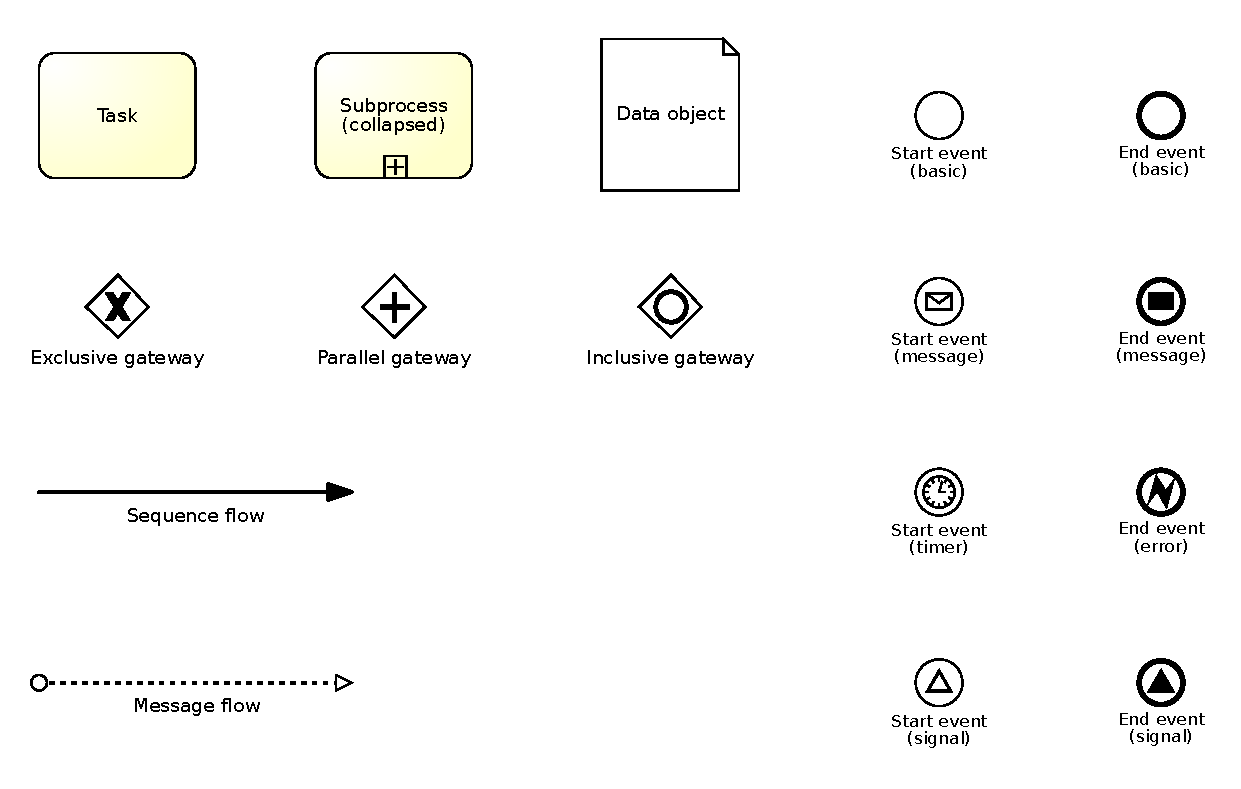
\includegraphics[width=\textwidth]{./images/bpmn_core_elements.pdf}
\caption{Graphical representation of basic BPMN elements}
\label{fig:bpmn_core_elements}
\end{figure}
Figure~\ref{fig:bpmn_core_elements} shows graphical representations of basic BPMN elements described above. Figure~\ref{fig:process_example} shows a simple example of a business process diagram. From the start event, the token is passed to the task ``Process the order''. Next task, ``Check out supplies status'' performs the data checkout, required for the exclusive gateway that appears next. When the commodity is available and the order can be completed, then the task "Accept the order" is carried out and whole process finishes. Otherwise, the process flow is split into two branches using parallel gateway. The two tasks performed next are ``Contact the supplier for restock'' and ``Inform the client about delay''. Next, the join parallel gateway synchronizes both paths and the process is finished.

\begin{figure}
	\centering
	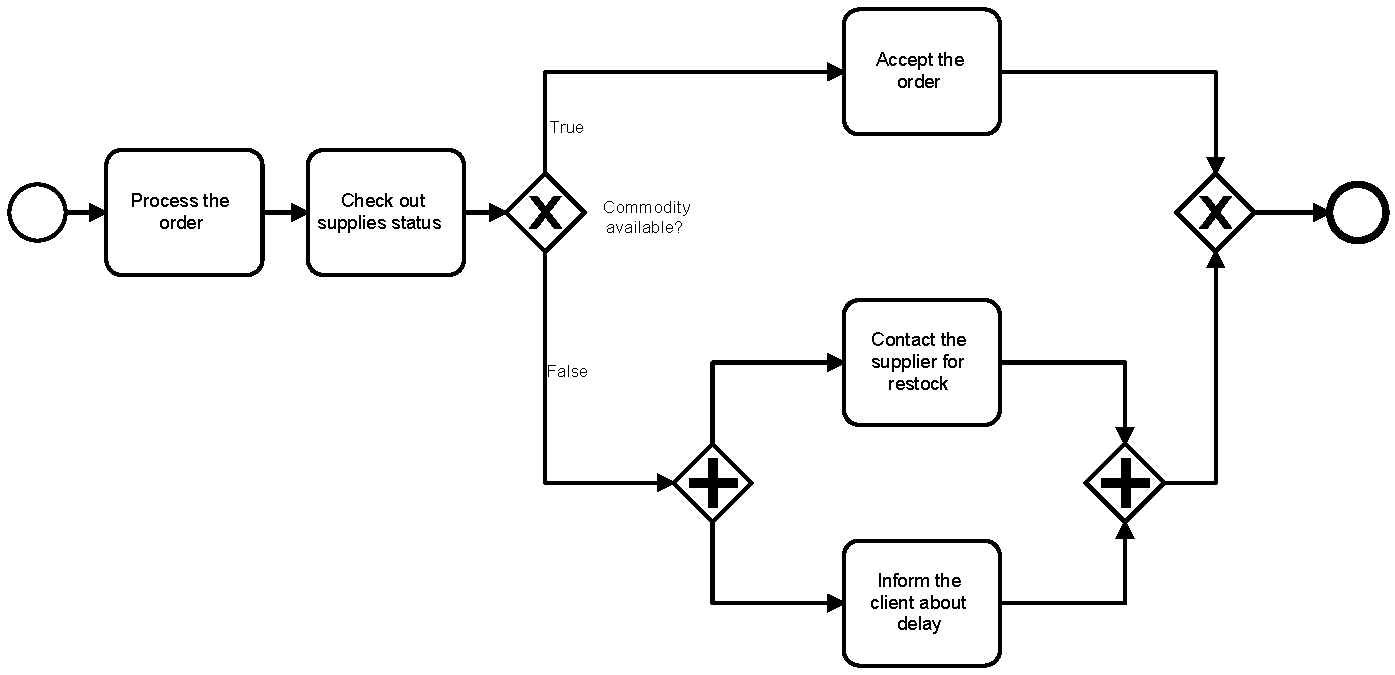
\includegraphics[width=\textwidth]{./images/process-example.pdf}
	\caption{An example of a simple BPMN business process}
	\label{fig:process_example}
\end{figure}

\section{Natural Language Processing}
\label{sec:nlp}
NLP~(\emph{Natural Language Processing}) is a branch of computer science, which combines elements of artificial intelligence and computational linguistics. NLP focuses on analysing and processing of natural language texts, in order to extract useful information and data, transforming them into an accessible for machines form. For the purpose of this thesis, two categories of NLP are important:
\begin{itemize}
	\item Syntax parsing -- grammatical analysis, parsing the syntax tree of the analysed text and part-of-speech (POS) tagging are the main concepts of this category,
	\item Semantic analysis -- extracting the meaning of words, which will be helpful in identifying the keywords, important from the business process point of view. 
\end{itemize}
There are many different tools which allows performing these tasks. A short description of both categories and the chosen tools will be given in the next subsections.

\subsection{Syntax parsing}
\label{subsec:syntax-parsing}
Syntax parsing focuses on determining the syntactic structure of a sentence (finding the grammatical relationships between words in analysed sentence) and part-of-speech tagging, which labels each word with a corresponding part of speech, based on its definition and context (i.e. adjacent words).\\
Examples of well-known tool used for the purpose of syntax parsing are NLTK (\emph{Natural Language Toolkit}), Stanford Parser or SpaCy parser project. For the purpose of syntax parsing, the SpaCy parser was chosen. SpaCy provides not only syntax parsing and POS tagging functionalities but is also able to perform tokenization, sentence decomposition, which will be useful for the purpose of this thesis.\\
The POS tagger provided by SpaCy utilizes two sets of Part-Of-Speech tags.  First one is based the OntoNotes 5 treebank~\cite{OntoNotes5},~\cite{ontnotes-2006}, which is based on earlier work, known as Penn Treebank~\cite{penntreebank-1993}. The secondary POS tag uses Universal Dependencies POS tags, which is simpler than the OntoNotes tags (for example there is only one tag for verbs -- OntoNotes provides tags for different tenses or persons).  Another important functionality of SpaCy is dependency parsing, which describes dependencies between words included in given sentence. Dependency parser used in SpaCy is based on ClearNLP project~\cite{ClearNLP}, with some extensions to dependency tags set. Figure~\ref{fig:sentence_example} shows an example of syntax tree, with Part-Of-Speech tag (from the OntoNotes tag set) and dependency tags, parsed from simple sentence ``This is an example of sentence, which can be parsed by SpaCy''.

\begin{figure}[ht]
	\centering
	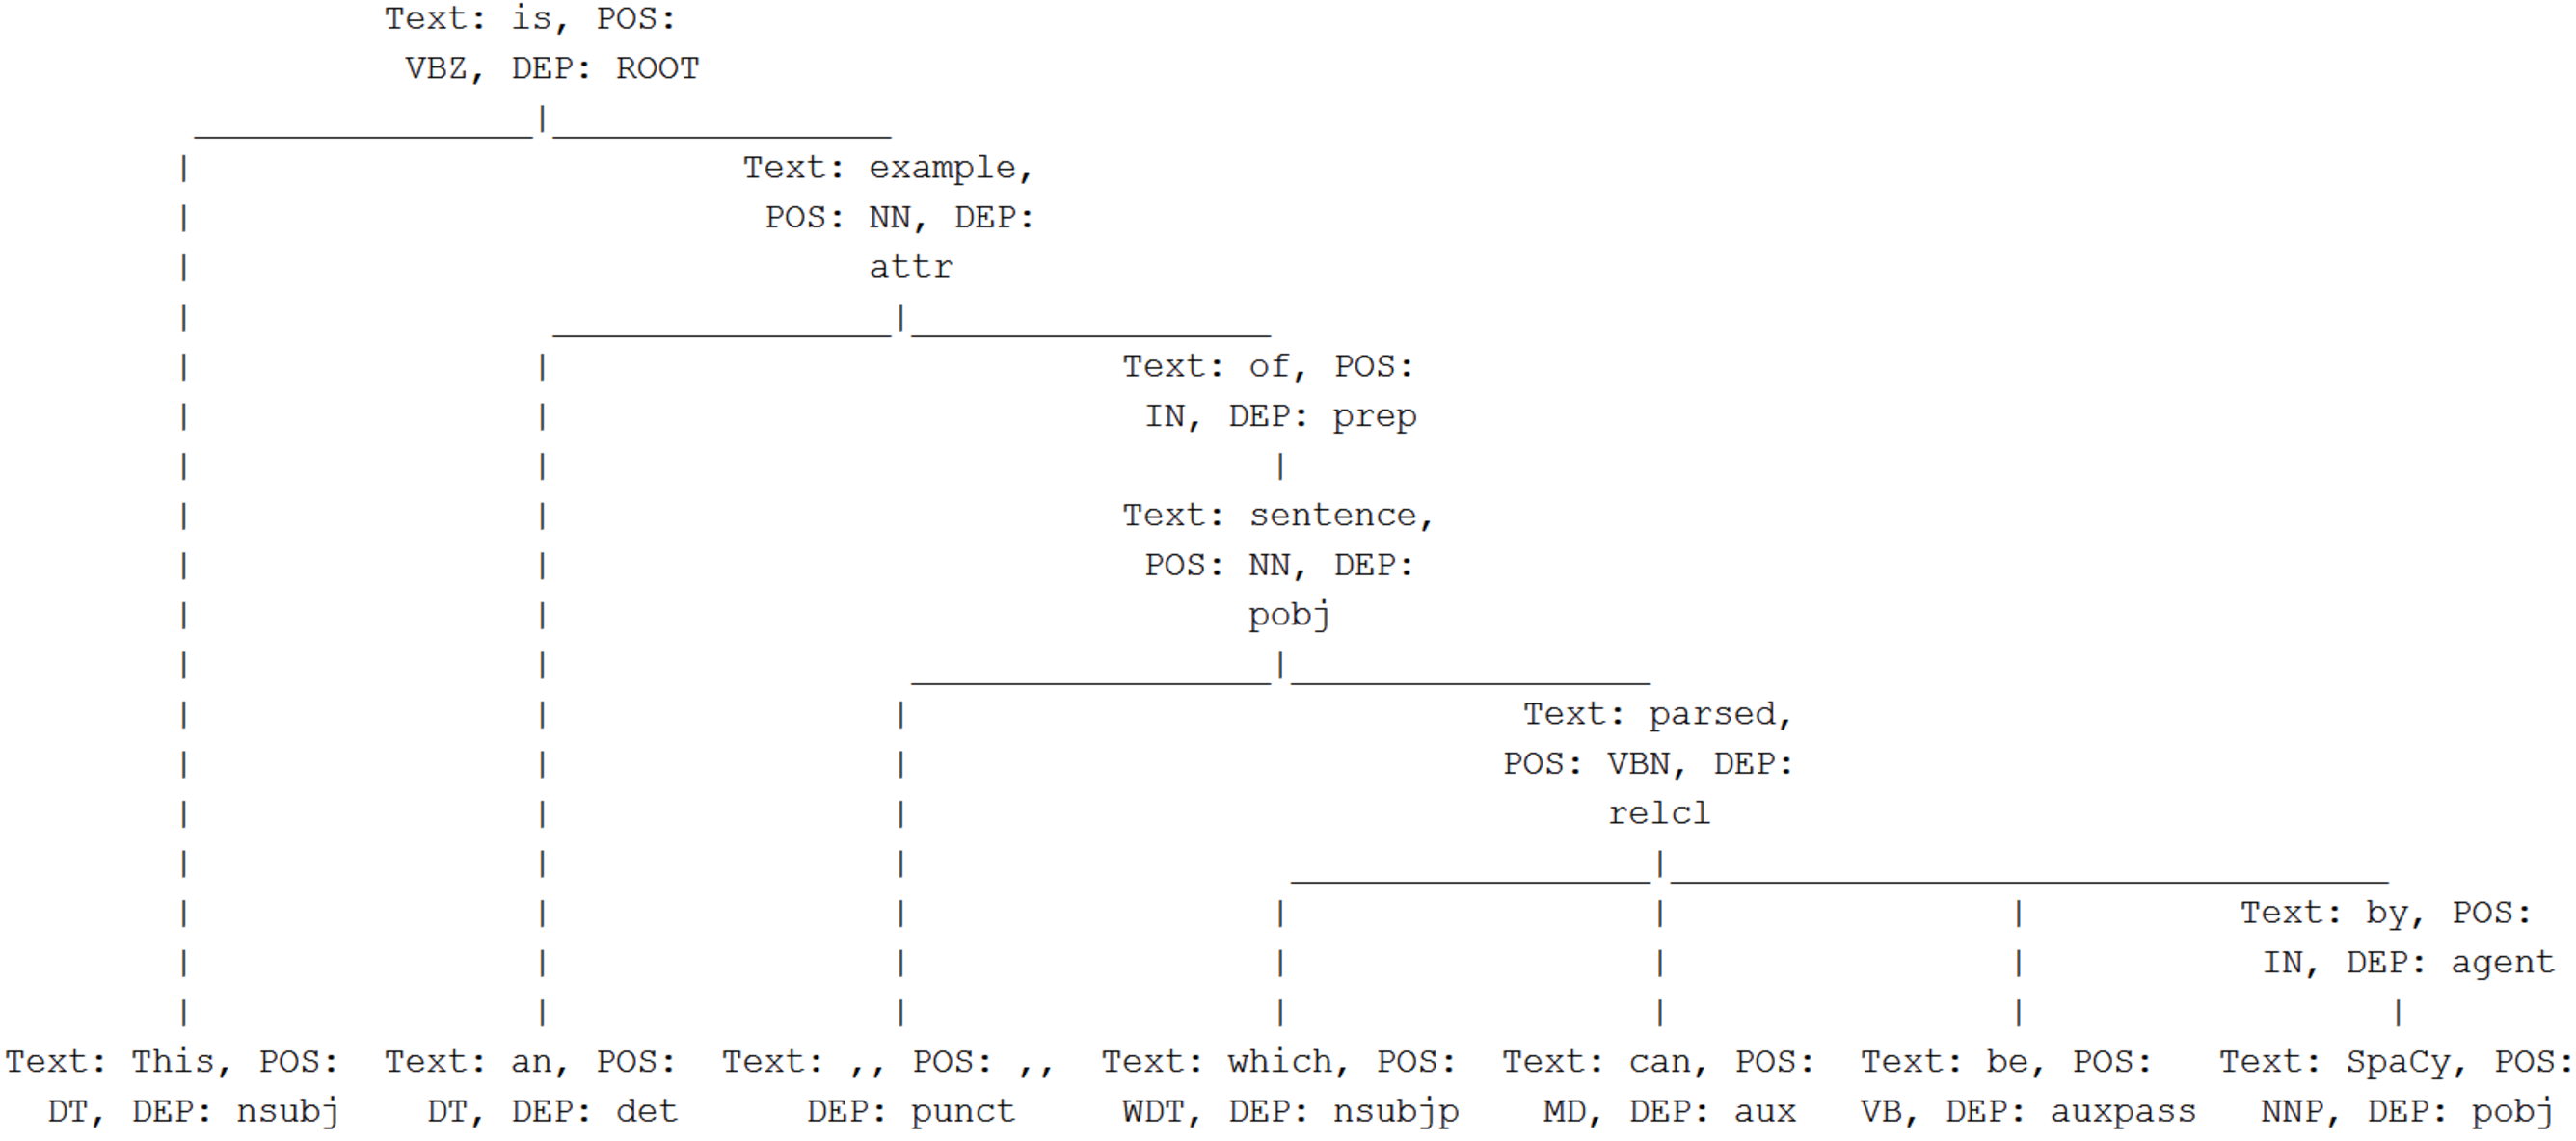
\includegraphics[width=\textwidth]{./images/sentence_example.pdf}
	\caption{An example of a sentence parsed by SpaCy}
	\label{fig:sentence_example}
\end{figure}

The dependency tag represents relation between child and parent in the tree. Notice that the word at the top of tree is tagged as ROOT.\\
Dependencies analysis is very helpful in determining the useful parts of natural language description, which can be later translated to BPMN process elements (mainly turning subject-verb-objects constructs into tasks). The full list of dependency tags available in SpaCy is described in Appendix~\ref{cha:dependencies-list}. Dependencies, which are used in proposed approach of translation, are shown in Table~\ref{table:dependencies}. This subset of dependencies should provide enough information to extract SVO (subject-verb-object) construct, which can be possibly translated into BPMN tasks. Auxiliary (\emph{aux}, \emph{auxpass}), modifier (\emph{amod}, \emph{neg}, \emph{prep}, \emph{poss}) and determiner dependencies can be used to extract additional words to better describe the extracted SVO.
\begin{table}[ht]
	\begin{tabular}{|l|c|}
		\hline
		Tag name & Description\\
		\hline
		\hline
		nsubj & nominal subject\\
		\hline
		nsubjpass & nominal passive subject\\
		\hline
		agent & agent\\
		\hline
		dobj & direct object\\
		\hline
		pobj & object of a preposition\\
		\hline
		iobj & indirect object\\
		\hline
		attr & attribute\\
		\hline
		conj & conjunct\\
		\hline
		compound & compound nouns or numbers\\
		\hline
		amod & adjectival modifier\\
		\hline
		aux & auxiliary\\
		\hline
		auxpass & auxiliary passive\\
		\hline
		neg & negation modifier\\
		\hline
		prep & prepositional modifier\\
		\hline
		poss & possession modifier\\
		\hline
	\end{tabular}	
	\caption{The subset of dependencies with definitions used in implemented prototype}
	\label{table:dependencies}
\end{table}
\subsection{Semantic analysis}
\label{subsec:semantic-analysis}
Semantic analysis focuses on interpreting the meaning of words in sentence. In the case of this thesis subject, semantic analysis allows us to eliminate information which was discovered during syntax analysis but is not useful from the business process point of view. As an example of such information, let us consider the sentences ,,Employee registers purchase'' and ,,Purchase is registered''. From the syntactic perspective, both of them should be treated as a subject-verb-object construct. Transforming them into BPMN tasks might be a correct decision -- in case of models made by business experts, it mostly depends on their point of view. Additional data, which can be extracted from these sentences, are information about people or inanimate entities (organizations, machines) involved in this task, which we will name as participants. In order to extract information about participants, we can validate if a given subject is synonymous to some general concept (for example ,,person'') which we assume to be a valid participant. In this case, ,,employee'' should be extracted as participant, but ,,purchase'' should be not.\\
Another use of semantic analysis is discovering some specific constructs, which indicate that some of the tasks are performed conditionally, excludes some other action or that a group of tasks can be executed simultaneously. This part of business process extraction will be explained further in section~\ref{cha:implementation}, which describes the algorithms in detail.\\
One of the most popular tools for semantic analysis is WordNet~\cite{word-net} -- a lexical database, which has been developed since 1985. WordNet contains information about sets of synonyms (synsets) for nouns, verbs, adjectives or adverbs. Different synsets are connected with each other by conceptual or lexical relations. Using WordNet, it is possible to analyse different semantic relations, such as synonyms, homonyms, hypernyms and other. This way, it should be possible to perform aforementioned analysis of extracted subjects and eliminate these that are not synonymous to some general concepts of participants.\\
Another useful functionality of WordNet is word stemming -- extracting the base meaning of word, removing lexemes. With the use of word stemming, it should be possible to produce normalized business process diagram and improve its readability and automatically create a unified tasks naming convention.

\section{Related work}
\label{sec:related}
In their recent publication~\cite{process-mining-state-of-the-art}, Terins and Thaler performed an analysis of current state-of-the-art in the field of mining process models from natural language text. A several different approaches were presented, some of which worked with some form of structuralized text (use cases, group stories), some with natural language description.
\begin{itemize}
\item Ghose, Koliadis and Chueng~\cite{proces-from-text-artefacts} proposed an approach for discovering a process model from text artefacts, which are described as \emph{documents such as memos, manuals, requirements documents, design documents, mission/vision statements, meeting minutes etc.} An extraction is performed by text pattern search (for example if/then pair, which indicates a conditional flow) and POS (\emph{Part-Of-Speech}) tagging combined with shallow parsing, which produces a syntax tree. This approach allows to discover parts of a larger model (called \emph{proto-models} by authors), rather than complete and sound model. Generated \emph{proto-models} can be compared in order to find similarities and remove redundant parts.

\item Goncalves et al.~\cite{mining-group-stories} presented a technique of obtaining process models from group stories. In the first phase, a text is tokenized in order to select words which can be useful for work-flow generation. Next, a POS tagging is performed. Finally, relevant entities are identified using a set of predefined patterns.
The produced BPMN model is not necessarily complete and sound -- it is assumed, that it will be later improved by process designer and team members, who created the group stories.
\begin{figure}[h!b]
	\centering
	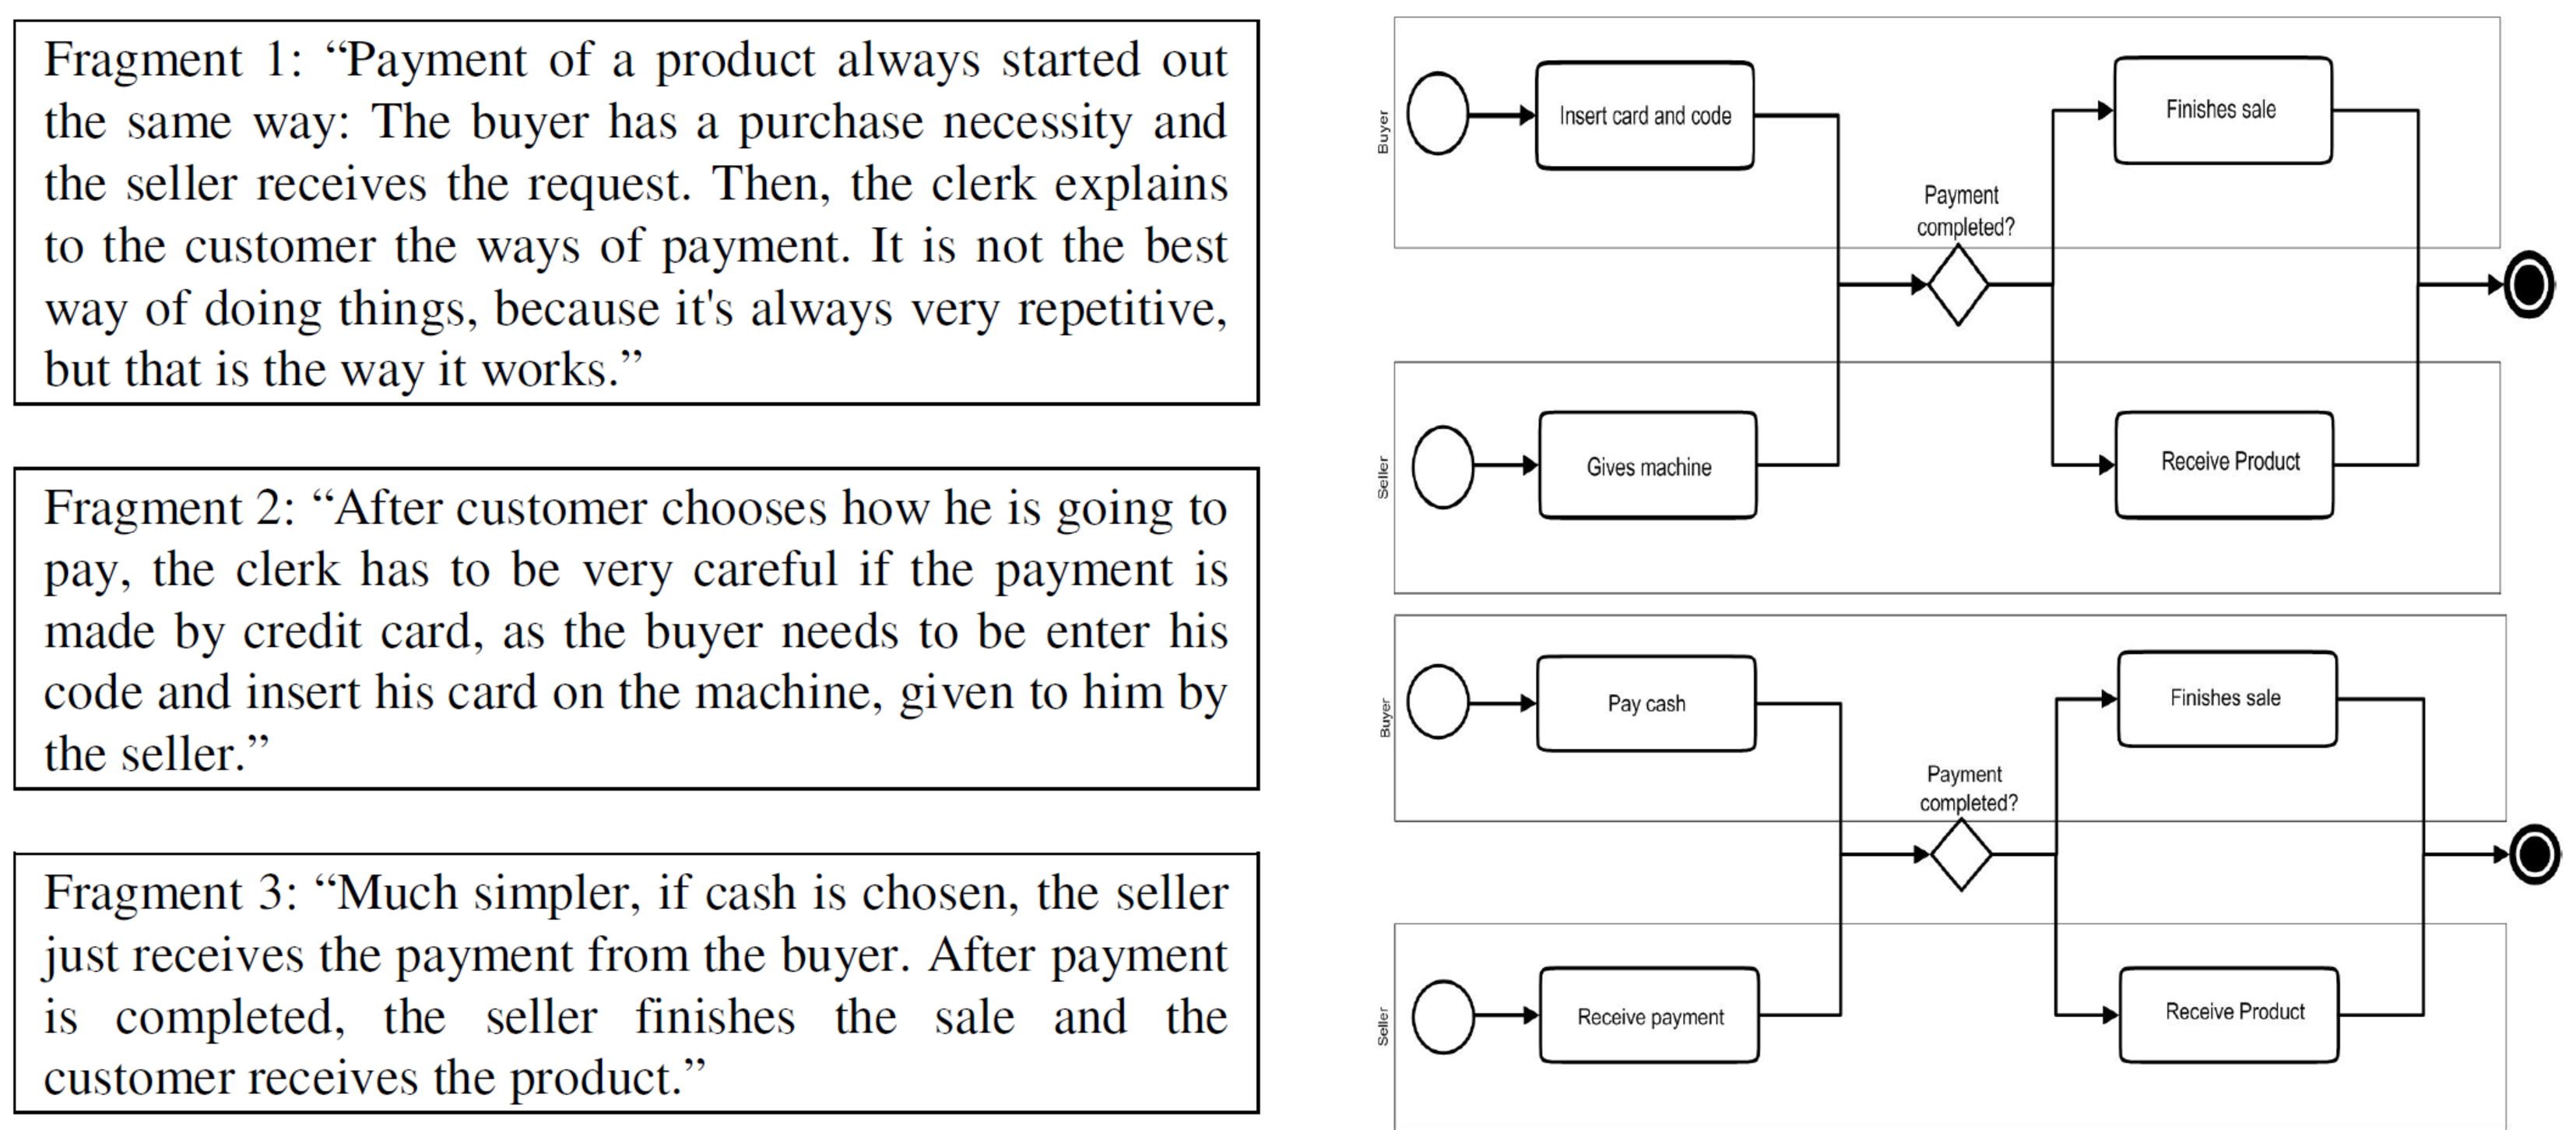
\includegraphics[width=\textwidth]{./images/goncalves_transform.pdf}
	\caption{Fragments of group story with corresponding BPMN elements generated by algorithm described in paper~\cite{mining-group-stories} (example obtained from article)}
	\label{fig:goncalves_example}
\end{figure}

\item Friedrich et al.~\cite{friedrich-2011} proposed an advanced approach, which uses a textual description of model. Such a description must follow some requirements -- a text cannot contain any questions and the described execution of a process must be sequential (any non-sequential jumps must be explicitly made). In the first step, a syntactical analysis (called \emph{Sentence Level Analysis} in the article) is performed, using Stanford NLP tools. Next, the semantic analysis (\emph{Text Level Analysis}), using WordNet and FrameNet databases, allows to identify relevant entities. Finally, the process model is generated (\emph{Process Model Generation} phase). Detailed flows for each phase are shown in Figures~\ref{fig:friedrich_sentence_analysis}~\ref{fig:friedrich_text_analysis}~\ref{fig:friedrich_process_generation}. The generated output is a sound and complete BPMN model, enriched with many additional elements (such as lanes, data sources), thanks to the rich text analysis. 
\end{itemize}
Several other methodologies for transforming natural language text into formalised models were proposed. Yue, Briand and Labiche~\cite{yue-2010} presented an automated approach to transform use case descriptions to UML Activity diagrams. This methodology requires that the use case descriptions has to follow some restriction rules. These rules can be classified into two groups -- the first group specifies constraints on the use of natural language, the second are requirement on the use of specific keywords to indicate the existence of control structures. In addition, the use case description explicitly lists all of the flows in the process (main and alternative) and each flow is a step-by-step description of a process.\\
Another approach in the field of generating formal models form natural language specification, proposed by Njonko and Abed~\cite{from-nl-to-model-via-sbvr}, uses SBVR (\emph{Semantics or Business Rules and Vocabulary}) as an intermediate layer for this transformation approach. It is suggested that using formalised model as an intermediate layer (in this case SBVR), it is possible to easily extend this approach for multiple models. The article presents an example of transformation from natural language business description into SQL executable query, which produces a database table that corresponds to business requirements.\\
In this section, the basic information about Business Process Management, BPMN notation and NLP was presented. Also, the SpaCy parser and the underlying technology of this tool were described. Next section describes the proposed approach to the problem and the implementation of prototype, which is based on SpaCy parser and utilizes the described NLP methods.
\begin{figure}[H]
	\centering
	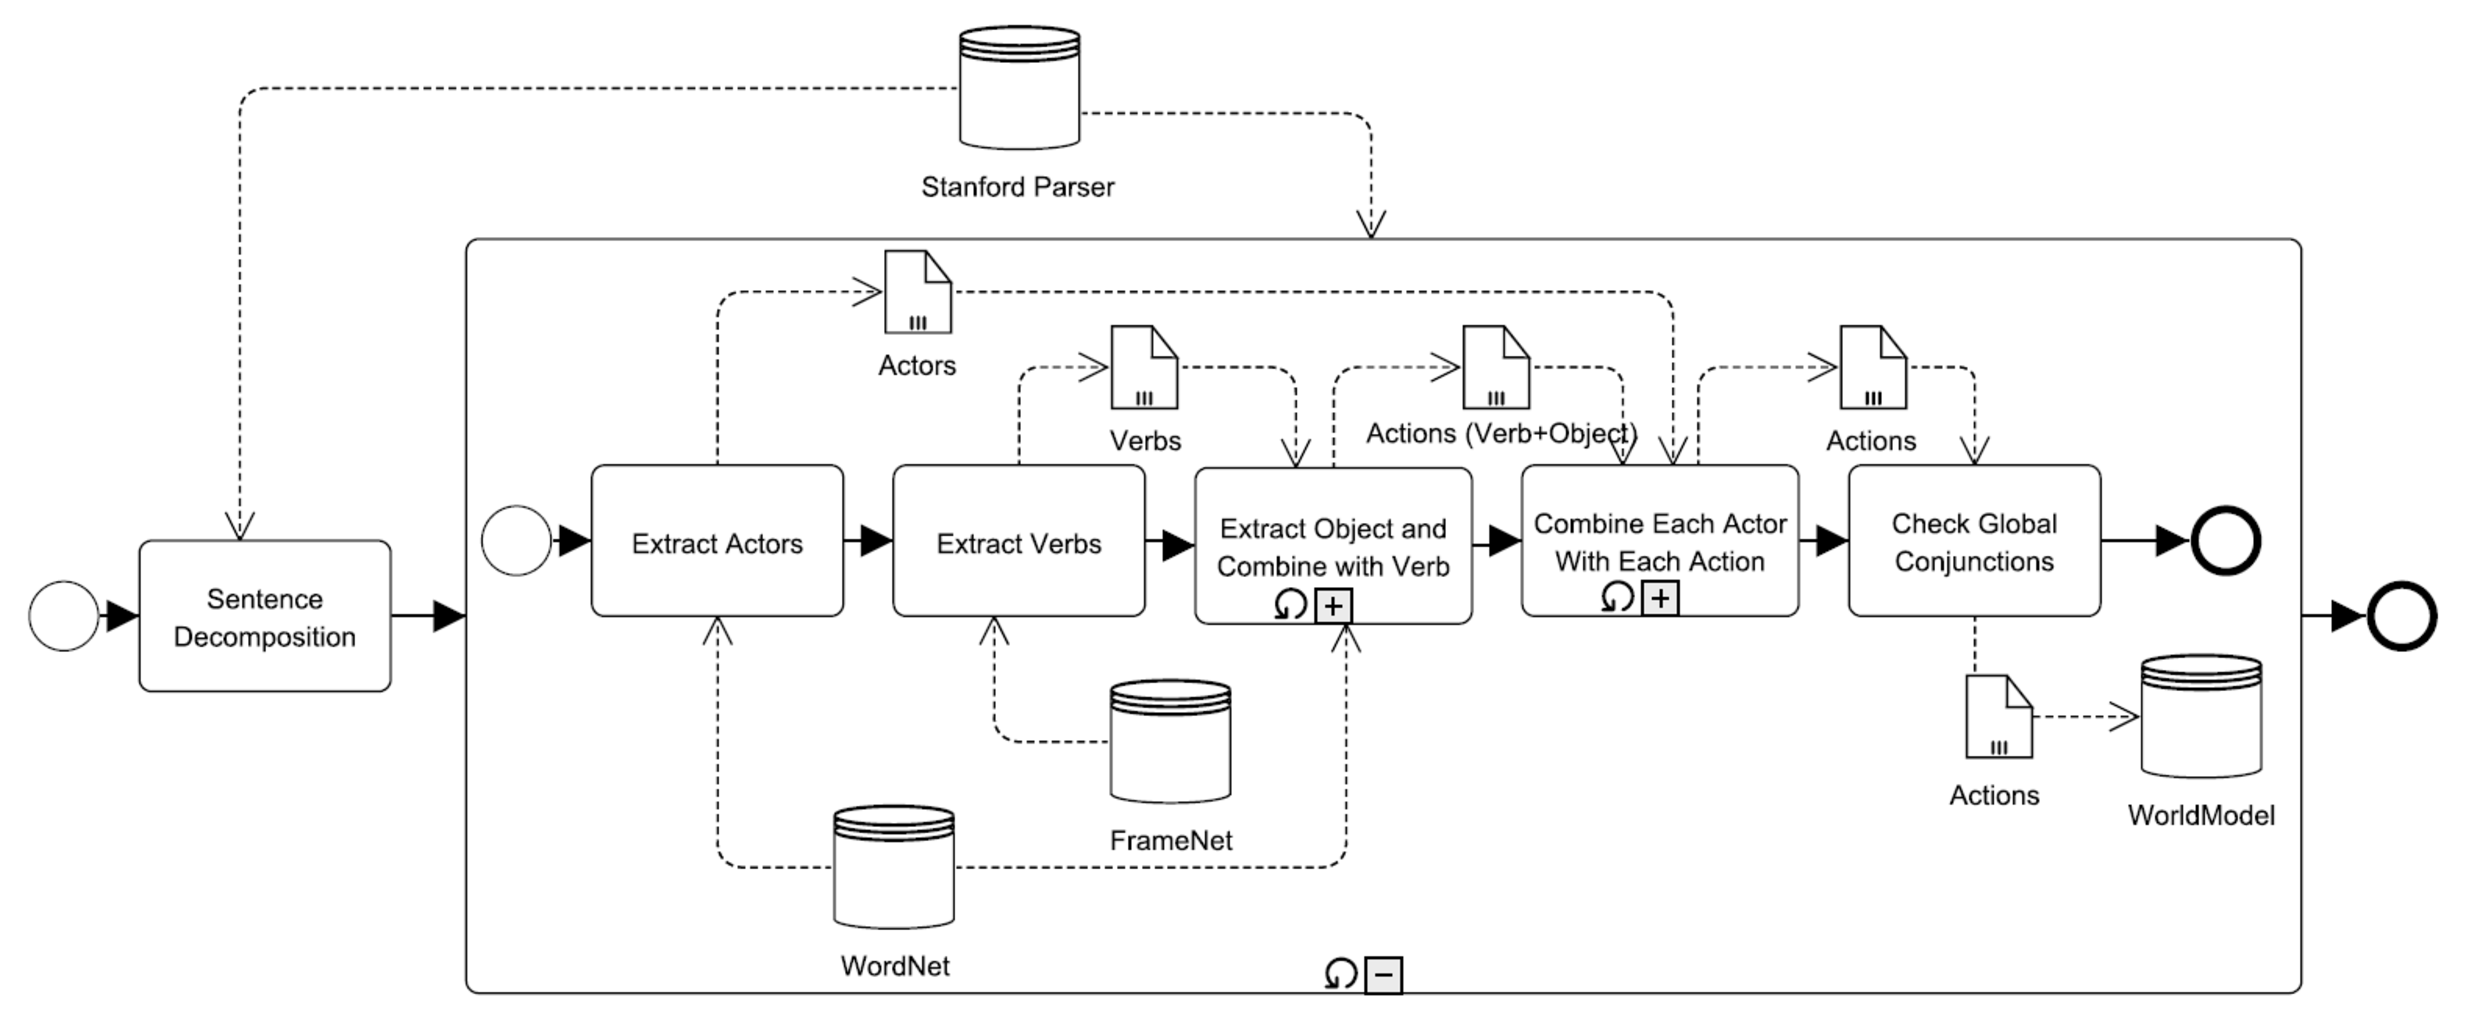
\includegraphics[width=\textwidth]{./images/friedrich_sentence_analysis.pdf}
	\caption{Detailed flow showing sentence analysis phase of transformation approach described in article~\cite{friedrich-2011} (diagram obtained from article)}
	\label{fig:friedrich_sentence_analysis}
\end{figure}
\begin{figure}[H]
	\centering
	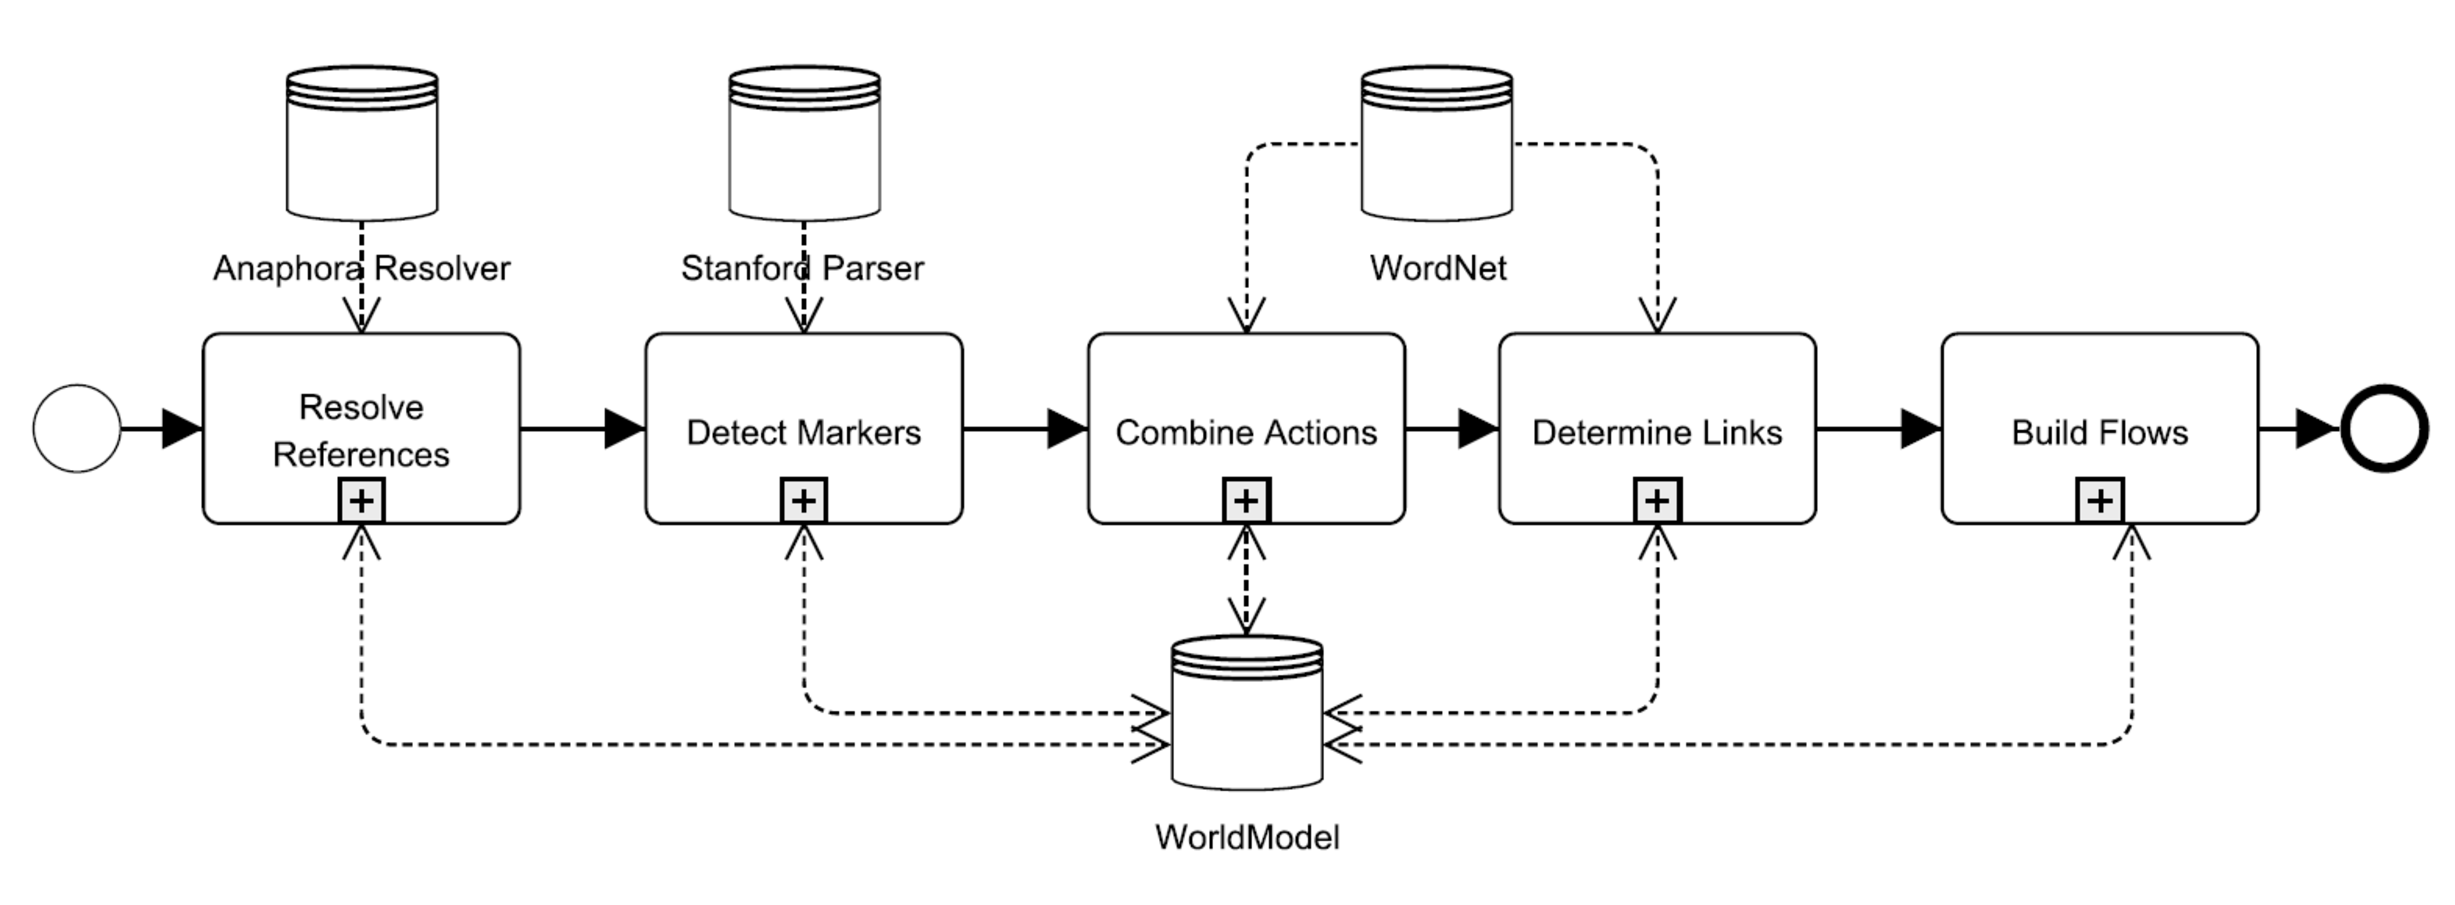
\includegraphics[width=\textwidth]{./images/friedrich_text_analysis.pdf}
	\caption{Detailed flow showing text analysis phase of transformation approach described in article~\cite{friedrich-2011} (diagram obtained from article)}
	\label{fig:friedrich_text_analysis}
\end{figure}
\begin{figure}[H]
	\centering
	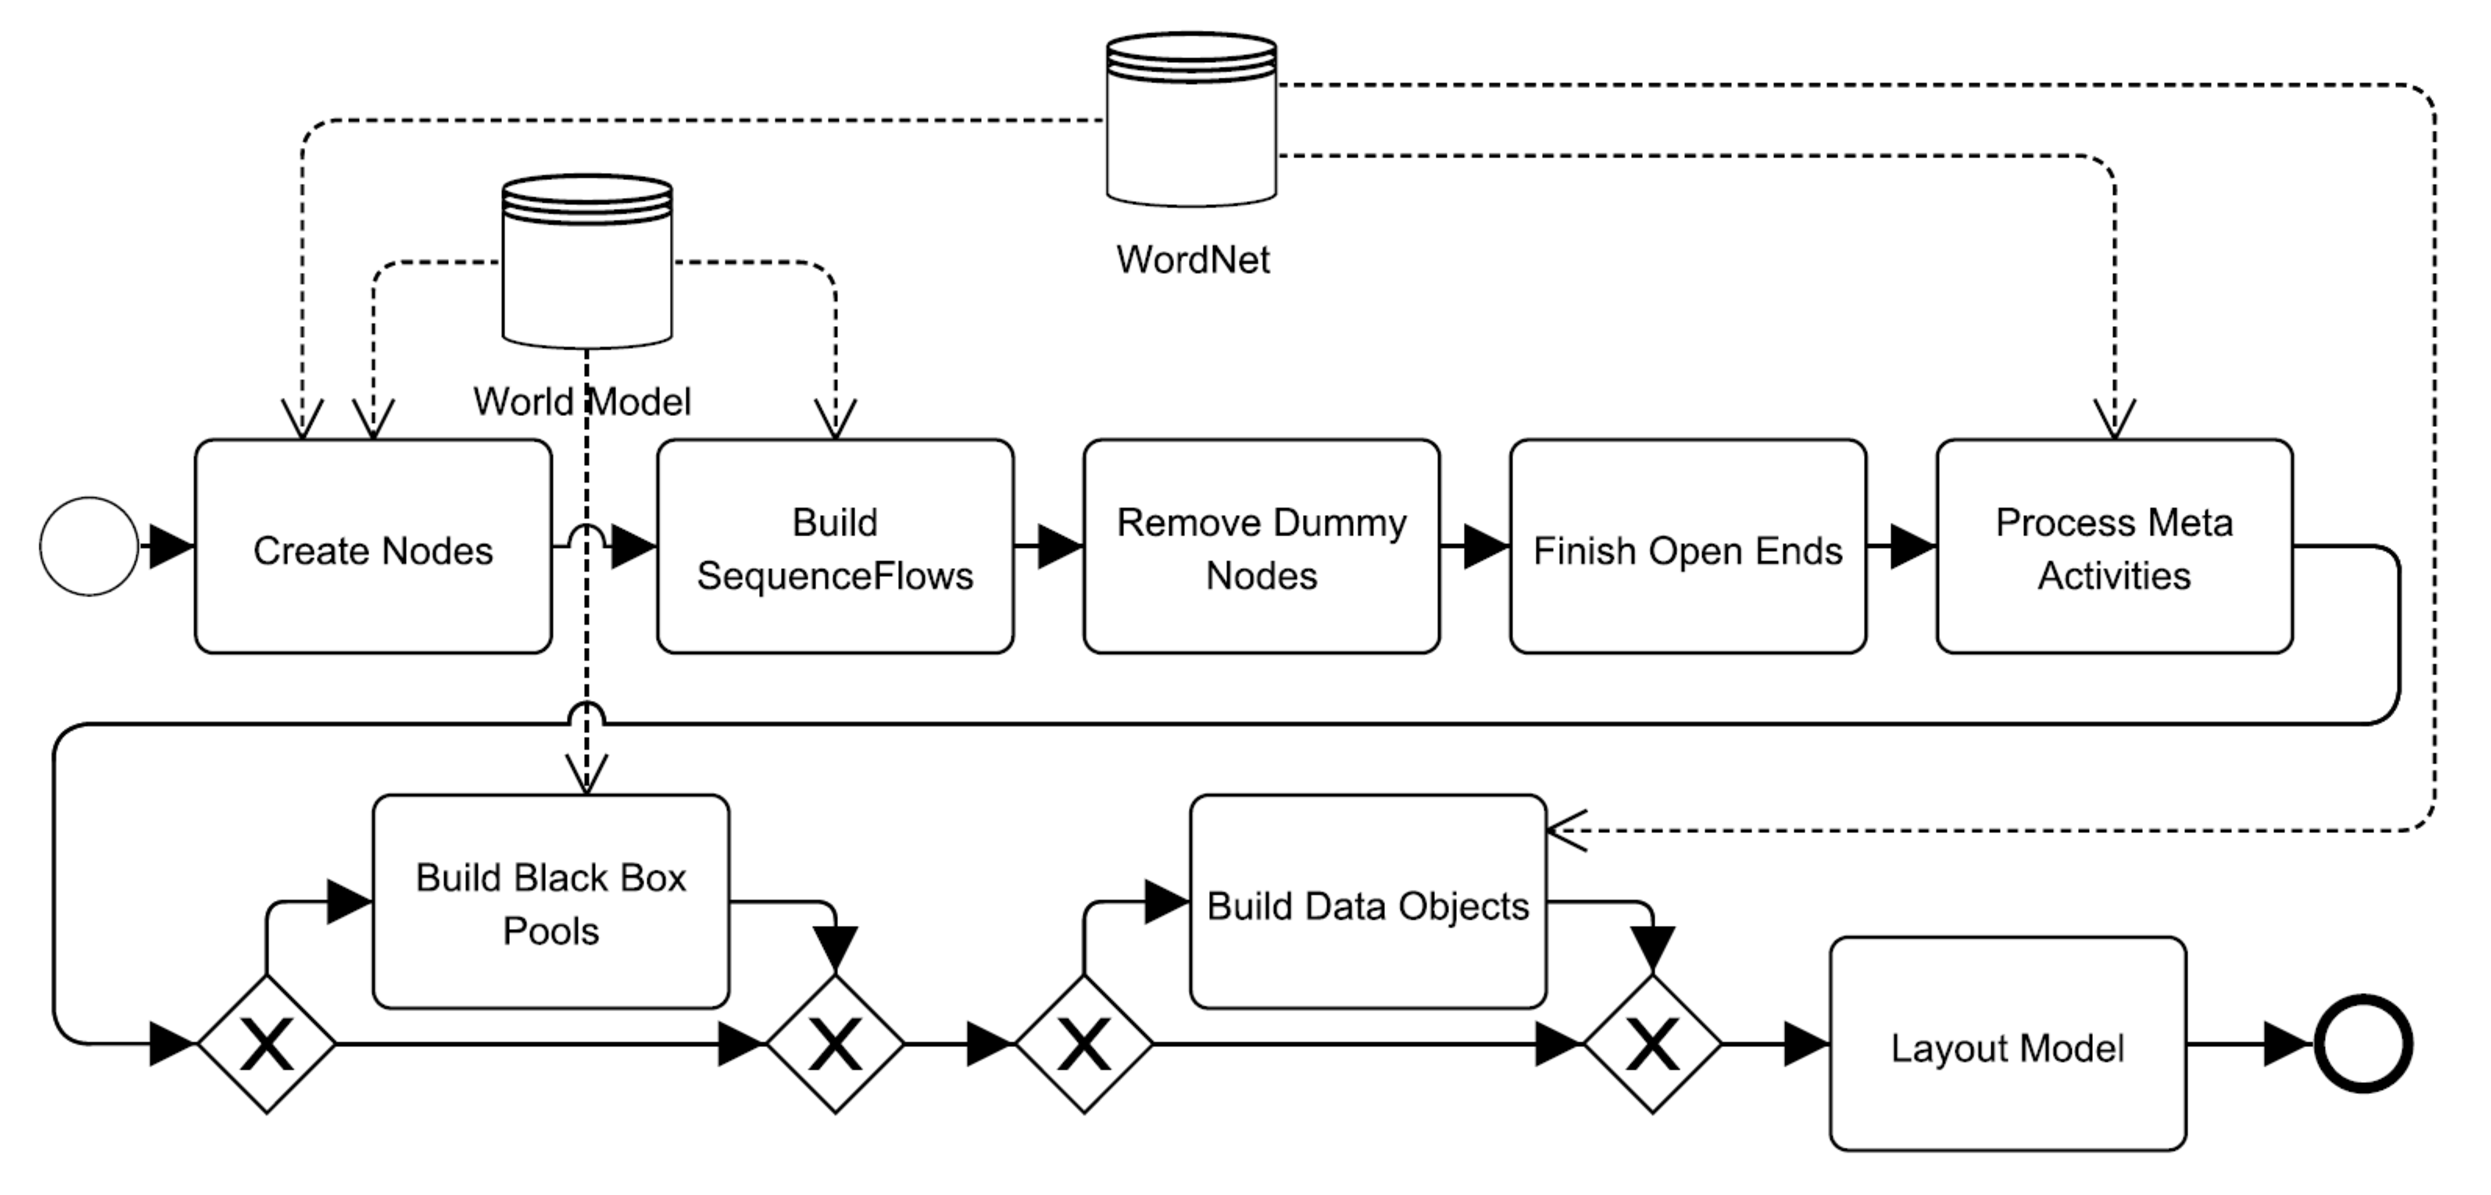
\includegraphics[width=\textwidth]{./images/friedrich_process_generation.pdf}
	\caption{Detailed flow showing process generation phase of transformation approach described in article~\cite{friedrich-2011} (diagram obtained from article)}
	\label{fig:friedrich_process_generation}
\end{figure}
\begin{figure}[H]
	\centering
	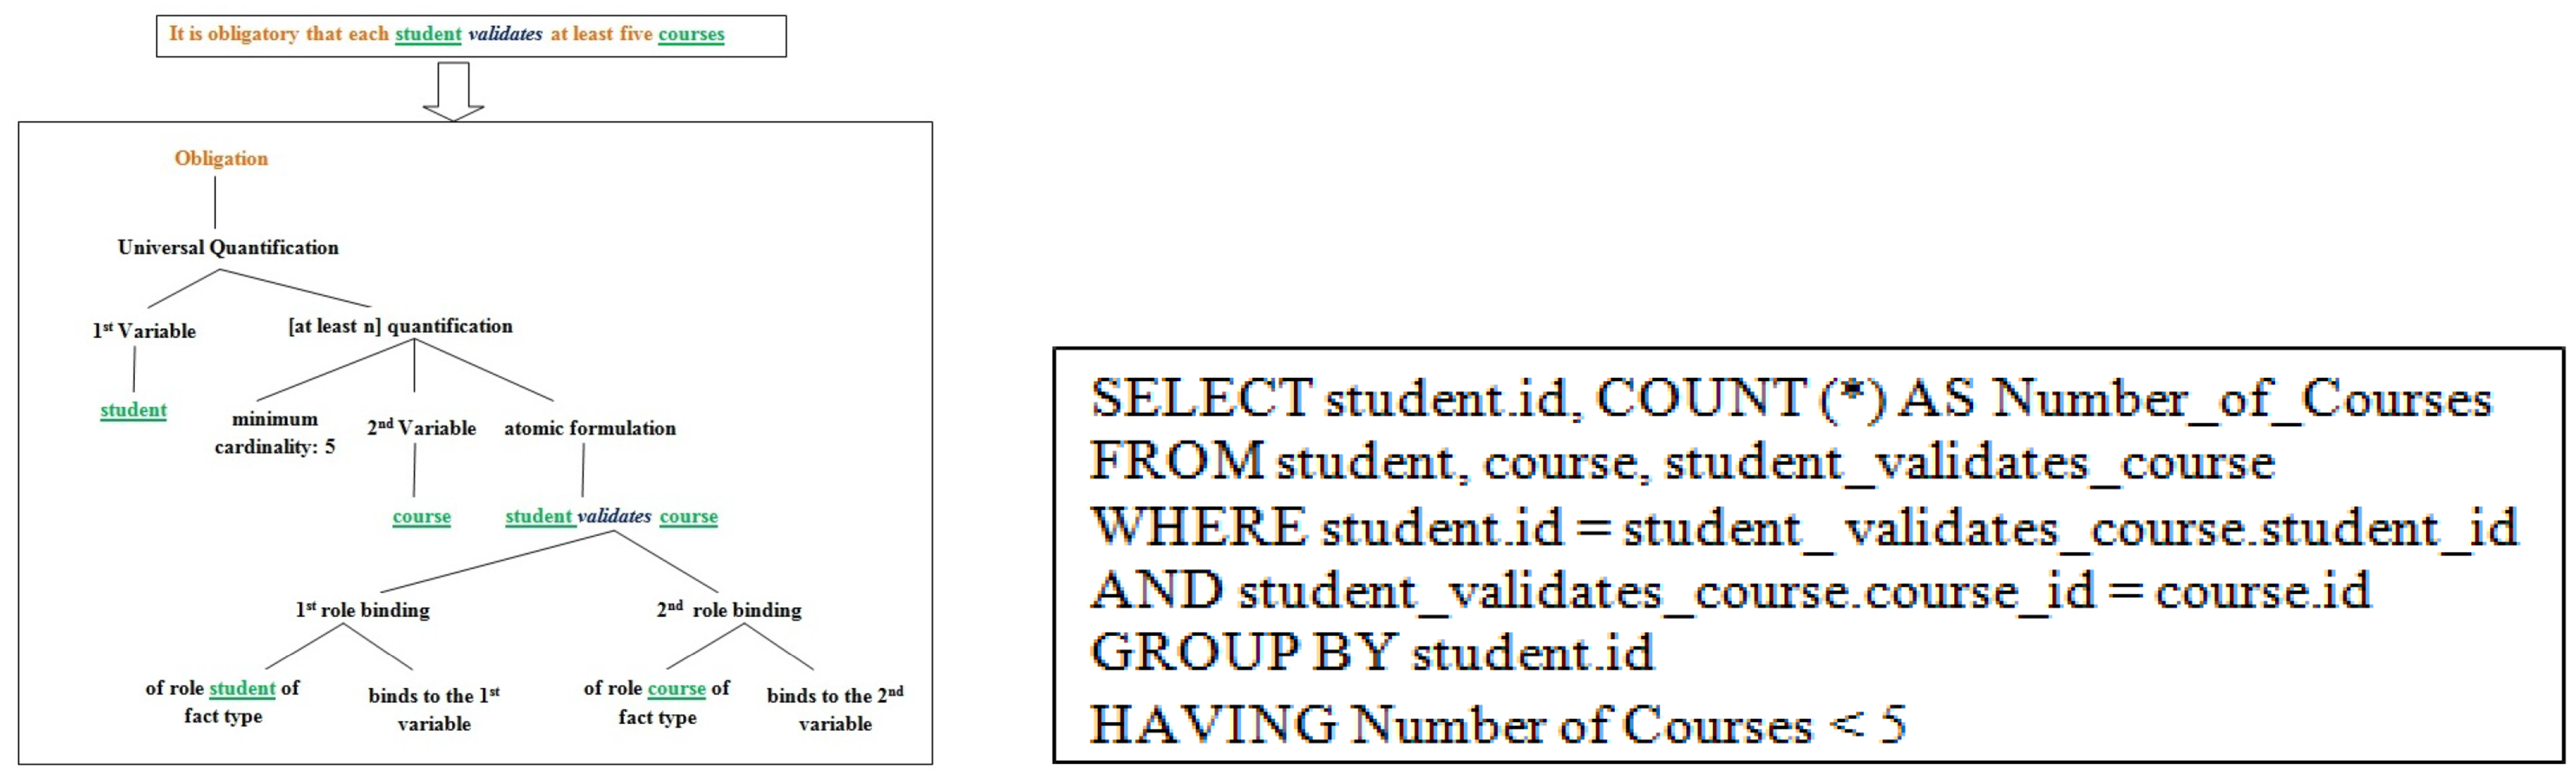
\includegraphics[width=\textwidth]{./images/njonko-example.pdf}
	\caption{An example of SQL query generated from business description, using method described in article~\cite{from-nl-to-model-via-sbvr} (pictures obtained from article)}
	\label{fig:njonko_example}
\end{figure}